\documentclass{amsart}
\usepackage[margin=1in]{geometry}
\usepackage{amsmath,amssymb,latexsym, tikz}

\newtheorem{thm}{Theorem}
\newtheorem{dfn}{Definition}
\newtheorem{lma}{Lemma}
\newtheorem{ex}{Example}
\newtheorem{clm}{Claim}


\newcommand{\CC}{\mathbb{C}}
\newcommand{\ZZ}{\mathbb{Z}}
\newcommand{\bfa}{\mathbf{a}}
\newcommand{\bfn}{\mathbf{n}}


\title{Two-Step Flag Varieties via\\ Compatible Subsets of Maximal Dyck Paths}

\author{Colleen Robichaux}
\author{Dylan Rupel}
\author{Harshit Yadav}

\begin{document}
  \begin{abstract}
    We show that the affine cells in certain quiver Grassmannians can be labeled by compatible subsets of maximal Dyck paths.
    The dimensions of these cells are shown to be computable combinatorially, verifying an analogue of a conjecture of the second author and Thorsten Weist.
  \end{abstract}
  \maketitle

  Say something about quiver Grassmannians

  Say something about compatible subsets of maximal Dyck paths

  Write $d_S=\sum\limits_{e<e'\in D_\bfn} d_S(e,e')$, where
  \[
    d_S(e,e')=
    \begin{cases}
      -1 & \text{if $e\in S\cap H_\bfn$ and $e'\in S\cap V_\bfn$;}\\
      1 & \text{if $e\in S\cap H_\bfn$ and $e'\in H_\bfn\setminus S$;}\\
      1 & \text{if $e\in V_\bfn\setminus S$ and $e'\in S\cap V_\bfn$;}\\
      0 & \text{otherwise.}
    \end{cases}
  \]
  The following is an analogue of \cite[Conjecture 5.21]{rupel-weist}.
  \begin{thm}
    Given a compatible subset $S\subset D_\bfn$ with $|S\cap H_\bfn|=n-k_2$ and $|S\cap V_\bfn|=k_1$, the affine cell in $Gr_{(k_1,k_2)}(\CC^n\leftarrow\CC^n)$ labeled by $S$ has dimension $d_S$.
  \end{thm}

  \section{Compatible Subsets of Maximal Dyck Paths}
  Given $\bfa\in\ZZ_{\ge0}^2$, let $D_\bfa$ denote the maximal Dyck path in the lattice rectangle with corner vertices $(0,0)$ and $\bfa$.
  That is, $D_\bfa$ is the lattice path that begins at $(0,0)$, takes East and North steps to end at $\bfa$ while never passing above the main diagonal of the rectangle.
  It is maximal in the sense that any lattice point lying above $D_\bfa$ also lies above the main diagonal.
  Write $H_\bfa$ (resp. $V_\bfa$) for the set of horizontal (resp. vertical) edges in $D_\bfa$.
  Note that the set $H_\bfa\sqcup V_\bfa$ has a natural ordering coming from the placement of edges along $D_\bfa$. 

  \begin{dfn}
    Fix $n\ge1$.
    A subset $S\subset H_\bfa\sqcup V_\bfa$ is \emph{$n$-compatible} if: for each $h\in H_\bfa$ and $v\in V_\bfa$ with $h<v$, there exists an edge $e$ with $h\le e\le v$ so that at least one of the following holds
    \[e\ne v \qquad \text{and} \qquad \big|\{v'\in V_\bfa:h\le v'\le e\}\big|=n\big|\{h'\in H_\bfa\cap S:h\le h'\le e\}\big|\]
    \[e\ne h \qquad \text{and} \qquad \big|\{h'\in H_\bfa:e\le h'\le v\}\big|=n\big|\{v'\in V_\bfa\cap S:e\le v'\le v\}\big|\]
  \end{dfn}

\section{Bijection with permutations}
Let $F(k_1,k_2;n)$ denote the $2$-step flag variety of tuples of vector subspaces $(V_1,V_2)$ of a fixed $n$-dimensional vector space $V$, where dim$(V_1)=k_1$, dim$(V_2)=k_2$ and $V_1\subset V_2$. The cohomology ring of the $2$-step flag variety is generated by the Poincare duals of the classes of Schubert varieties in $F(k_1,k_2)$. These Schubert varieties are parameterized by permuatations $w\in W(k_1,k_2)\subset S_n$ where
\[W(k_1,k_2):=\{w\in S_n \ | \ w(i)<w(i+1) \ \mbox{ if } \ i\in [n]\backslash \{k_1,k_2\}\}\]
We will call these permuataions as $2$-grassmannian permutations. 

It is well known that the dimension of the Schubert variety corresponding to the permutation $w$ (denoted $\sigma_w$) is equal to the number of inversions of $w$: 

\[\ell(w):=\#\{1\leq i<j\leq n \ | \ w(i)>w(j)\}.\]

\begin{ex}\label{ex:2step}
For $n=8$, we see $w=25378146$ is $2$-grassmanian since if $i\not\in\{2,5\}$, $w(i)<w(i+1)$, so $k_1=2$ and $k_2=5$. 

%Similarly $v=46123578$ is $2$-grassmanian where, so $k_1=2$ and $k_2=8$. 
\end{ex}

Also define 
\[ S(k_1,k_2):= \{ S\in D_\bfn  \ | \  |S\cap H_\bfn|=k_1, |S\cap V_\bfn|=n-k_2\} \]
%|S(k_1,k_2)\cap H_n|=n-k_2 and |S(k_1,k_2)\cap V_n|=k_1.


%%%%%%feel free to change notation if you see a better choice for phi 
For $k_1,k_2$ fixed, we define a map $\phi_{k_1,k_2}$ between $W(k_1,k_2)$ and $S(k_1,k_2)$ as follows. Suppose that $w =(w_1,w_2,\ldots,w_n)  \in W(k_1,k_2)$. Define $S_w:=\phi_{k_1,k_2} (w)$ to be the subset of $D_\bfn$ such that $S_w \cap H_\bfn=\{ H_{w_{k_2 +1}},H_{w_{k_2 +2}}, \ldots, H_{w_n} \}$ and $S_w \cap V_\bfn = \{V_{w_1},V_{w_2},\ldots,V_{w_{k_1}}\}$  

\begin{ex}\label{ex:phiW}%%%%%fix notation of V_n as set and V_n as edge
For $w$ as in Example \ref{ex:2step}, we would have $S_w \cap H_\mathbf{8}=\{ H_{w_{6}},H_{w_{7}}, H_{w_8} \}=\{ 1,4, 6 \}$ and $S_w \cap V_\mathbf{8} = \{V_{w_1},V_{w_2}\}= \{2,5\}$. Below is $D_{\mathbf 8}$ with $S_w$ in red. \begin{center} 
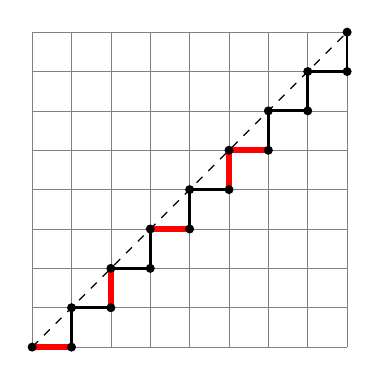
\begin{tikzpicture}[scale=0.5]
(0,0) rectangle +(8,8);
\draw[help lines] (0,0) grid +(8,8);
\draw[dashed] (0,0) -- +(8,8);
% \coordinate (prev) at (8,0);
\draw [color=red,line width=2] (0,0)--(1,0);
\draw [line width=1] (1,1)--(2,1);
\draw [line width=1] (2,2)--(3,2);
\draw [color=red,line width=2] (3,3)--(4,3);
\draw [line width=1] (4,4)--(5,4);
\draw [color=red,line width=2] (5,5)--(6,5);
\draw [line width=1] (6,6)--(7,6);
\draw [line width=1] (7,7)--(8,7);

\draw [line width=1] (1,0)--(1,1);
\draw [color=red,line width=2] (2,1)--(2,2);
\draw [line width=1] (3,2)--(3,3);
\draw [line width=1] (4,3)--(4,4);
\draw [color=red,line width=2] (5,4)--(5,5);
\draw [line width=1] (6,5)--(6,6);
\draw [line width=1] (7,6)--(7,7);
\draw [line width=1] (8,7)--(8,8);

% \draw [color=red, line width=1] (8,0)--(9,0)--(10,0)--(10,1)--(10,2)--(13,2)--(13,3)--(13,5);

\draw (0,0) node [scale=0.3, circle, draw,fill=black]{};
\draw (1,1) node [scale=0.3, circle, draw,fill=black]{};
\draw (2,2) node [scale=0.3, circle, draw,fill=black]{};
\draw (3,3) node [scale=0.3, circle, draw,fill=black]{};
\draw (4,4) node [scale=0.3, circle, draw,fill=black]{};
\draw (5,5) node [scale=0.3, circle, draw,fill=black]{};
\draw (6,6) node [scale=0.3, circle, draw,fill=black]{};
\draw (7,7) node [scale=0.3, circle, draw,fill=black]{};
\draw (8,8) node [scale=0.3, circle, draw,fill=black]{};

\draw (1,0) node [scale=0.3, circle, draw,fill=black]{};
\draw (2,1) node [scale=0.3, circle, draw,fill=black]{};
\draw (3,2) node [scale=0.3, circle, draw,fill=black]{};
\draw (4,3) node [scale=0.3, circle, draw,fill=black]{};
\draw (5,4) node [scale=0.3, circle, draw,fill=black]{};
\draw (6,5) node [scale=0.3, circle, draw,fill=black]{};
\draw (7,6) node [scale=0.3, circle, draw,fill=black]{};
\draw (8,7) node [scale=0.3, circle, draw,fill=black]{};

 \end{tikzpicture}
 \end{center}
\end{ex}


%Take $\phi_{k_1,k_2}(id):=S_{id}$ where $S_{id}\cap H_n=\{H_1,\ldots,H_{n-k_1}\}$ and $S_{id}\cap V_n=\{V_{n-k_2},\ldots,V_{n}\}$. 

%Show we can get everything by applying simple transp. to id, all remaining in $W(k_1,k_2)$.

%Then any other $w\in W(k_1,k_2)$

\begin{lma}\label{lma:mapCompat}
If $w\in W(k_1,k_2)$, then $S_w$ is a compatible subset of $D_\bfn$.
\end{lma}
\begin{proof}
Since $w$ is a permutation, $i\neq j$ means that $w_i\neq w_j$. Thus, it is straightforward to see that the horizontal and vertical edges are always at different positions. Therefore, $S_w$ is a compatible subset of $D_\bfn$.
\end{proof}

\begin{lma}\label{lma:bij}
$\phi$ is a bijection.
\end{lma}
\begin{proof}
It is easy to see that $\phi$ is an injective map since $w$ $2$-grassmanian uniquely determines $w_{k_1+1},\ldots,w_{k_2}$, given $w_{1},\ldots,w_{k_1}$ and $w_{k_2+1},\ldots,w_{n}$. Given any compatible subset $S\in S(k_1,k_2)$, we construct a permutation $w\in W(k_1,k_2)$ such that $S_w=S$. Suppose that $S\cap V_\bfn = \{V_{i_1},\ldots,V_{i_{k_1}} \}$ and $i_1<\ldots<i_{k_1}$. Also suppose $S\cap H_\bfn=\{ H_{j_1},H_{j_2},\ldots, H_{j_{n-k_2}} \}$ and that $j_1<\ldots<j_{n-k_2}$. Finally, suppose $\{m_1, \ldots,m_{n-k_1-k_2}\} = [n]\backslash \{i_1,\ldots,i_{k_1},j_1,\ldots,j_{n-k_2} \}$ sorted in ascending order.

Then we define $w$ as follows
\[
w_k= 
\begin{cases}
  i_k & \text{if $k\leq k_1$};\\
  m_{k-k_1} & \text{if $k_1< k \leq k_2 $;}\\
  j_{k-k_2} & \text{if $k > k_2 $;}\\
\end{cases}
\]
It follows from the construction of $w$ that $S_{w}=S$.
\end{proof}




\begin{lma}\label{lma:lenMatch}
If $S_w=S$, then $\ell(w)=d_S$.
\end{lma}
\begin{proof}
First we give a new definition of $\widetilde{d}_S$. For $e=H_i$ let $n(e):=V_i$, and if $e'=V_i$ let $n(e'):=H_i$

 Then $\widetilde{d}_S=\sum\limits_{e<e'\in D_\bfn} \widetilde{d}_S(e,e')$, where
  \[
    \widetilde{d}_S(e,e')=
    \begin{cases}
     % -1 & \text{if $e\in S\cap H_\bfn$ and $e'\in S\cap V_\bfn$;}\\
      1 & \text{if $e\in S\cap H_\bfn$,  $e'\in H_\bfn\setminus S$, and $n(e')\in V_\bfn\setminus S$;}\\
      1 & \text{if $e\in V_\bfn\setminus S$ and $e'\in S\cap V_\bfn$;}\\
      0 & \text{otherwise.}
    \end{cases}
  \]


By Lemma \ref{lma:mapCompat}, $S$ is a compatible subset. Thus if $e\in S\cap H_\bfn$ then $n(e)\in V_\bfn\setminus S$, and similarly if $e\in S\cap V_\bfn$ then $n(e)\in H_\bfn\setminus S$. 
Thus $\widetilde{d}_S={d}_S$.


We see $\ell(w)=\sum\limits_{1\leq i<j\leq n} \ell(i,j)$
where 
 \[
    \ell(i,j)=
    \begin{cases}
      1 & \text{if } w_i>w_j\\
      0 & \text{otherwise.}
    \end{cases}
  \]
 
 Let $w^{(1)}:=w_1,\ldots,w_{k_1}$, $w^{(2)}:=w_{k_1+1},\ldots,w_{k_2}$, and $w^{(3)}:=w_{k_2+1},\ldots,w_{n}$. 
 
Let $\Phi':[n]\times [n]\rightarrow D_\bfn\times D_\bfn$ where $\Phi'$ is defined by the following:


 \[
    \Phi'(i,j)=
    \begin{cases}
      (V_{w_i},V_{w_j}) & \text{if } i\in[1,\ldots,k_1]\\
      (H_{w_i},H_{w_j}) & \text{if } i\in[k_2+1,\ldots,n].
    \end{cases}
  \]

 Then define $\Phi:[n]\times [n]\rightarrow D_\bfn\times D_\bfn$ for $i<j$ such that if $\Phi'(i,j)=(e,e')$, then 
\[
    \Phi(i,j)=
    \begin{cases}
      (e,e') & \text{if } w_i<w_j\\
      (e',e) & \text{if } w_i>w_j.
    \end{cases}
  \]
 
\begin{clm}\label{clm:pairMatch}
For $1\leq i<j\leq n$,  the following hold:
\begin{itemize}
    %\item $\Phi$ is injective
    \item[(i)] $\ell(i,j)=\widetilde{d}_S(\Phi(i,j))$
    \item[(ii)] If $(e,e')\not\in$ Im$\Phi$, $\widetilde{d}_S(e,e')=0$.
\end{itemize}
\end{clm}

If Claim \ref{clm:pairMatch} holds, \[\ell(w)=\sum\limits_{1\leq i<j\leq n} \ell(i,j)=\sum\limits_{1\leq i<j\leq n} \widetilde{d}_S(\Phi(i,j))=\sum\limits_{e<e'\in D_\bfn} \widetilde{d}_S(e,e')=\widetilde{d}_S={d}_S,\]
so the lemma is proven.


\noindent\emph{Proof of Claim \ref{clm:pairMatch}:}
The proof of (i) follows by casework of $i,j$ in intervals $I_1=[1,\ldots,k_1]$, $I_2=[k_1+1,\ldots,k_2]$, and $I_3=[k_2+1,\ldots,n]$.\\ 

\noindent {\sf Case 1:}($i,j\in I_m$ where $1\leq m\leq 3$) 
Since $w\in W(k_1,k_2)$, if $i,j\in I_m$ then $w_i<w_j$, so $\ell(i,j)=0$. 
If $m=1$, $\Phi(i,j)=(V_{w_i},V_{w_j})$. By the definition of $S$, $V_{w_i}\in S\cap V_\bfn$, so 
$\widetilde{d}_S(V_{w_i},V_{w_j})=0$.
If $m=2$, $\Phi(i,j)=(H_{w_i},H_{w_j})$. By the definition of $S$, $H_{w_i}\not\in S\cap H_\bfn$, so 
$\widetilde{d}_S(H_{w_i},H_{w_j})=0$.
Finally if $m=3$, $\Phi(i,j)=(H_{w_i},H_{w_j})$. By the definition of $S$, $H_{w_i},H_{w_j}\in S\cap H_\bfn$, so 
$\widetilde{d}_S(H_{w_i},H_{w_j})=0$.\\


\noindent {\sf Case 2:}($i\in I_1$ and $j\in I_{2}\cup I_3$)
If $w_i<w_j$, then $\ell(i,j)=0$.
Further $\Phi(i,j)=(V_{w_i},V_{w_j})$, so 
$\widetilde{d}_S(\Phi(i,j))=0$ since $V_{w_i}\in S\cap V_\bfn$.
If $w_i>w_j$, then $\ell(i,j)=1$.
Further $\Phi(i,j)=(V_{w_j},V_{w_i})$, so since $V_{w_j}\in V_\bfn\setminus S$ and $V_{w_i}\in S\cap V_\bfn$,
$\widetilde{d}_S(\Phi(i,j))=1$.\\

\noindent {\sf Case 3:}($i\in I_2$ and $j\in I_{3}$)
If $w_i<w_j$, then $\ell(i,j)=0$.
Further $\Phi(i,j)=(H_{w_i},H_{w_j})$, so 
$\widetilde{d}_S(\Phi(i,j))=0$ since $H_{w_i}\in H_\bfn\setminus S$.
If $w_i>w_j$, then $\ell(i,j)=1$.
Further $\Phi(i,j)=(H_{w_j},H_{w_i})$, so 
$\widetilde{d}_S(\Phi(i,j))=1$ since $H_{w_j}\in S\cap H_\bfn$, $H_{w_i}\in H_\bfn\setminus S$, and $V_{w_i}\in V_\bfn\setminus S$.


This clearly exhausts all cases of $(i,j)$ where $i<j$. 
Thus it remains to check that if $(e,e')\not\in$Im$\Phi$, then $\widetilde{d}_S(e,e')=0$.

Let $U\subset D_\bfn\times D_\bfn$ containing elements of the form:
\begin{itemize}
    \item $(H_k, V_{k'})$,
    \item $(V_k, H_{k'})$,
    \item $(V_k, V_{k'})$ where $k<k'\in I_2\cup I_3$,
    \item $(H_k, H_{k'})$ where $k\in I_1\cup I_2$,
    \item $(H_k, H_{k'})$ where $k\in I_3$, $k'\in I_1$,
\end{itemize}
 where $1\leq k'\leq k\leq n$.
Using the definitions of $S$ and $\Phi$, is straightforward to check that $D_\bfn\times D_\bfn\setminus $Im$\Phi\subseteq U$. Further it is clear from the definition of $\widetilde{d}_S$ that if $(e,e')\in U$, $\widetilde{d}_S(e,e')=0$. Thus the result follows.
\end{proof}






\end{document}